\section{Dynamic Visual Querying}\label{sec:visualQuery}
To facilitate astronomers' discovery of time intervals similar to a ROI/SOI (\textbf{G3}) or those validating specific hypotheses (\textbf{G4}), 
TimeTubesX provides two different user-initiative visual query interfaces: query-by-example (QBE) and query-by-sketch (QBS).
Both are designed to help users identify similar patterns of interest (\textbf{T4}), and our matching algorithm allows for a fuzzy search (\textbf{T5}).

\subsection{Query-by-Example}\label{sec:QBE}
While the TimeTubes view helps users analyze time variations,
it remains challenging for users to build queries for multi-dimensional, time-dependent data.
Our QBE interface allows users to specify a notable behavior as a ROI with simple interactions through the TimeTubes or scatterplots views.
Users can pick a part of time-series data as an input for a query as well as flexibly select specific variables that should be queried about to reflect their intentions. 
This allows users to easily and intuitively search long-term datasets for interesting patterns with minimal required user inputs.

Fig.~\ref{fig:querySpecificationPanel} (B) shows our QBE interface.
To facilitate visual verification by users, a time interval selected through the TimeTubes or scatterplots views in (2, red highlight) is automatically extracted and displayed in the query panel (1).
After selecting the initial time interval, users can then fine-tune and adjust their query by selecting the variables that should be queried about. 
This is crucial for effective support of queries on multi-dimensional data.
Based on the selected variables, 
our system interactively updates the appearance of the 3D tube for the selected time interval in (1), visually encoding only currently selected variables.
For example, when users remove the variable $C$ from the query, the tube loses color variation and becomes a gray tube, as shown in (1).
After defining the query, users can adjust the main parameters (e.g., normalization and polar coordinates options) for our matching algorithm (see Section~\ref{sec:matchingAlgorithm}). 

\textsf{Experimental results.\ } We verified the effectiveness of our QBE method using our synthetic data.
The red circular patterns in Fig.~\ref{fig:synthesisData}~(b) have a similar shape but different time lengths, scales, or locations in the Stokes plane.
We used the leftmost red time interval in (b) as an input query, as shown in Fig.~\ref{fig:QBEDemodata}~(a).
We selected $q$ and $u$ as active variables and used the normalization and polar coordinates options to detect time intervals with different scales or different positions.
The length of the target time interval was set to 5 to 20 days.
We used $\rm{DTW}_{\rm D}$ as a distance function.
Note that we detail the options and parameters related to the matching process in Section~\ref{sec:matchingAlgorithm}.
Fig.~\ref{fig:QBEDemodata}~(b) shows the top three results of our QBE in (a).
The color of the rectangles corresponds to those used in Fig.~\ref{fig:synthesisData}~(b).
We were able to detect all time intervals with a similar shape in our synthetic dataset.
Note that the time interval specified for the query itself is omitted from the results.

\begin{figure}[tb]
    \centering
    \begin{minipage}{0.24\linewidth}
        \centering
        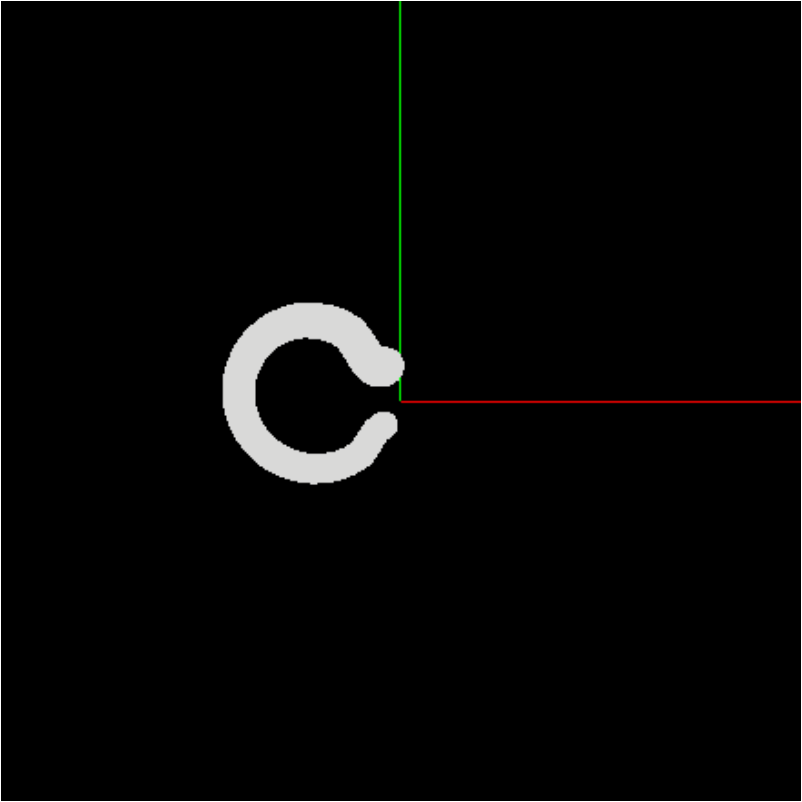
\includegraphics[width=.99\linewidth]{figures/QBE.png}
        \footnotesize{\sf (a)~Query.}
    \end{minipage}
    \begin{minipage}{0.75\linewidth}
        \centering
        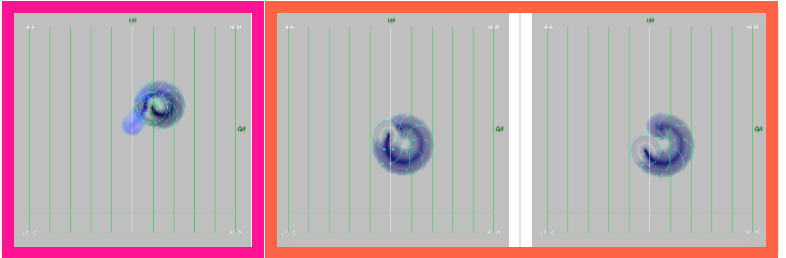
\includegraphics[width=.99\linewidth]{figures/QBEdemodataResults_revised.png}
        \footnotesize{\sf(b)~Results for the query in (a).}
    \end{minipage}
    \caption{QBE for our synthetic dataset in Fig.~\ref{fig:synthesisData}. 
        We chose the time interval with a small circular pattern (the leftmost red pattern in Fig.~\ref{fig:synthesisData}~(b)) for a query in (a). 
        Our method precisely extracted other time intervals with small circular patterns (the two red patterns from the right in Fig.~\ref{fig:synthesisData}~(b)).
        The outline color corresponds to the color in Fig.~\ref{fig:synthesisData}~(b).}
    \label{fig:QBEDemodata}
\end{figure}
\subsection{Query-by-Sketch}\label{sec:QBS}
TimeTubesX also allows users to query their data by manually drawing time variation patterns onto a 2D sketch interface.
Our QBS interface provides an intuitive and accessible way for users to specify patterns for multi-dimensional, semi-structured, time-dependent blazar datasets and validate their high-level hypotheses.
Rouxel et al.~\cite{Rouxel2014} state that an input trajectory by analog gestures is characterized by three dimensions: space, time, and force.
To realize intuitive interactions, 
we use space to determine the $x$ and $y$ positions of the stroke
and use either drawing speed or drawing pressure to define the stroke width 
so that users can describe time variations of multiple dimensions simultaneously.
Using the drawing speed option, the longer a cursor stays on a single point, the wider the curve at the point becomes.
To take into account other variables that are not described in sketching gestures, 
our QBS interface allows users to assign filtering constraints for each variable.
Thus, a sketch-based query for multi-dimensional, semi-structured, time-dependent data can be built with a single gesture
without sketching time variation patterns several times.

Fig.~\ref{fig:querySpecificationPanel} (C) shows the QBS query specification panel.
First, users define which variables are assigned to the $x$ and $y$ axes of the sketch pad and the stroke width (see panel (5)).
Second, they sketch a time variation pattern on a 2D sketch pad UI (3),
where the stroke is shown in black and its width is shown in blue.
Afterward, our system automatically beautifies the input stroke by fitting it to a cubic Bezier curve with as few segments as possible by using the \texttt{\small simplify} method in Paper.js~\cite{paper_framework}.
After their initial drawing, users can further adjust the sketch
by adding, removing, or moving control points or by changing the stroke width.
Users are also allowed to assign filtering constraints to each of the control points on the stroke, as shown in part (4).
They can define value ranges for each variable at the control point, which the algorithm will subsequently use when evaluating the query.

\begin{figure}[tb]
    \centering
    \begin{minipage}{0.49\linewidth}
        \centering
        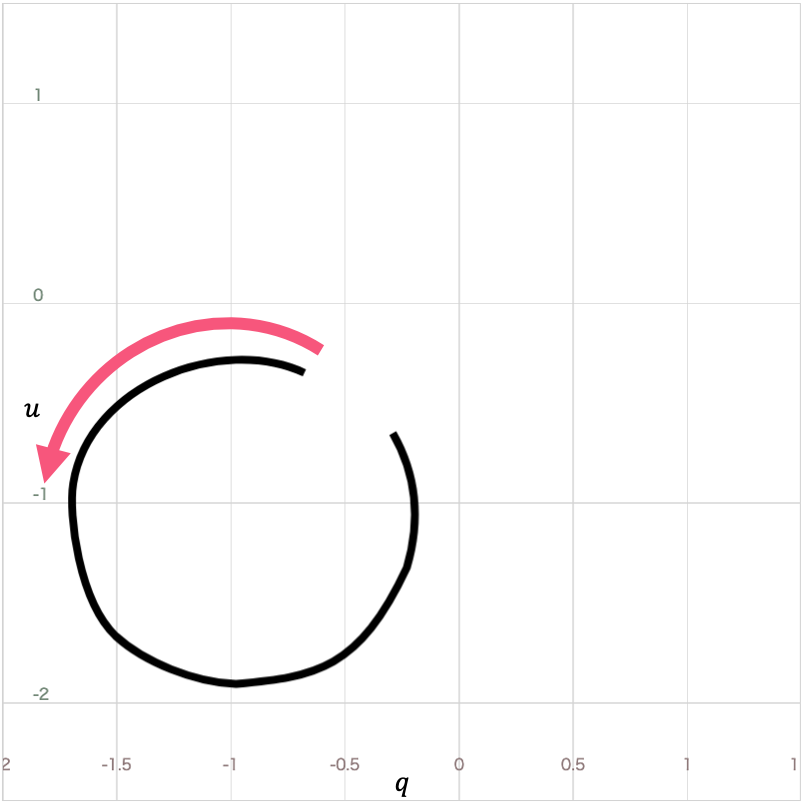
\includegraphics[width=.9\linewidth]{figures/QBSSketchwithoutWidth.png}
    \end{minipage}
    \begin{minipage}{0.49\linewidth}
        \centering
        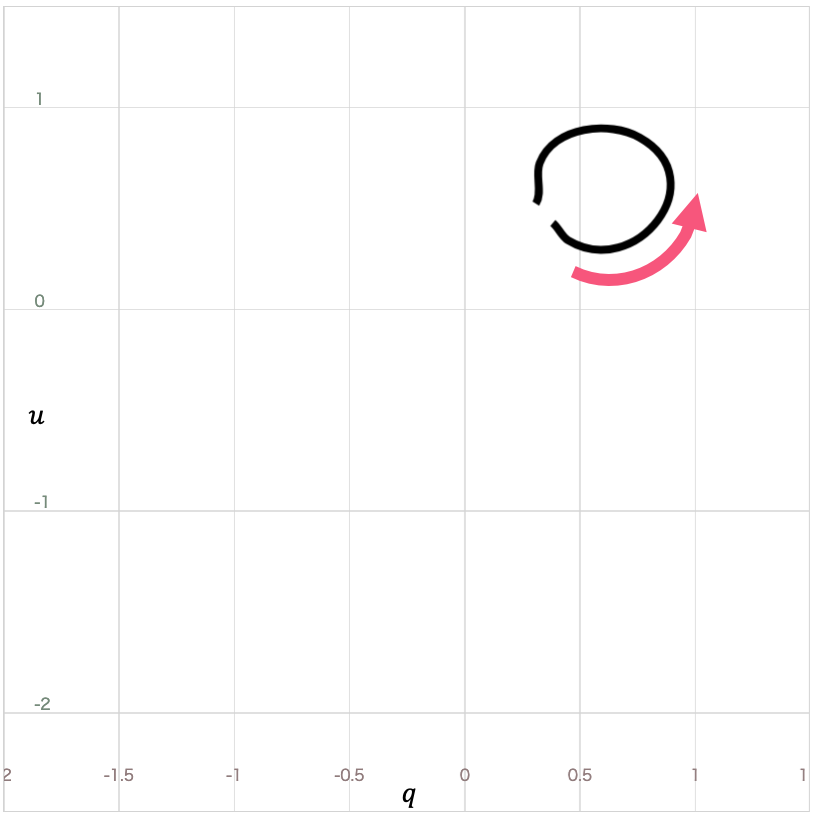
\includegraphics[width=.9\linewidth]{figures/QBSResultQuerywithoutWidth.png}
    \end{minipage}
    \begin{minipage}{0.49\linewidth}
        \centering
        \footnotesize{\sf (a)~A hand-drawn sketch query for a small circular pattern.}
    \end{minipage}
    \begin{minipage}{0.49\linewidth}
        \centering
        \footnotesize{\sf (b)~A sketch based on the upper left result in (c). 
        }
    \end{minipage}
    \begin{minipage}{0.49\linewidth}
        \centering
        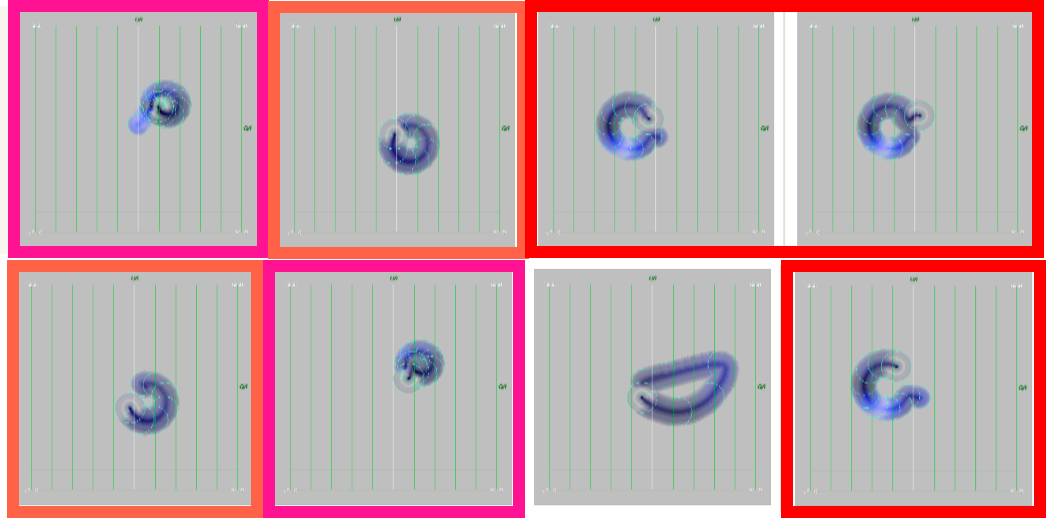
\includegraphics[width=.99\linewidth]{figures/QBSResultsHanddrawn_revised.png}\\
        \footnotesize{\sf (c)~Results for the query in (a).}
    \end{minipage}
    \begin{minipage}{0.49\linewidth}
        \centering
        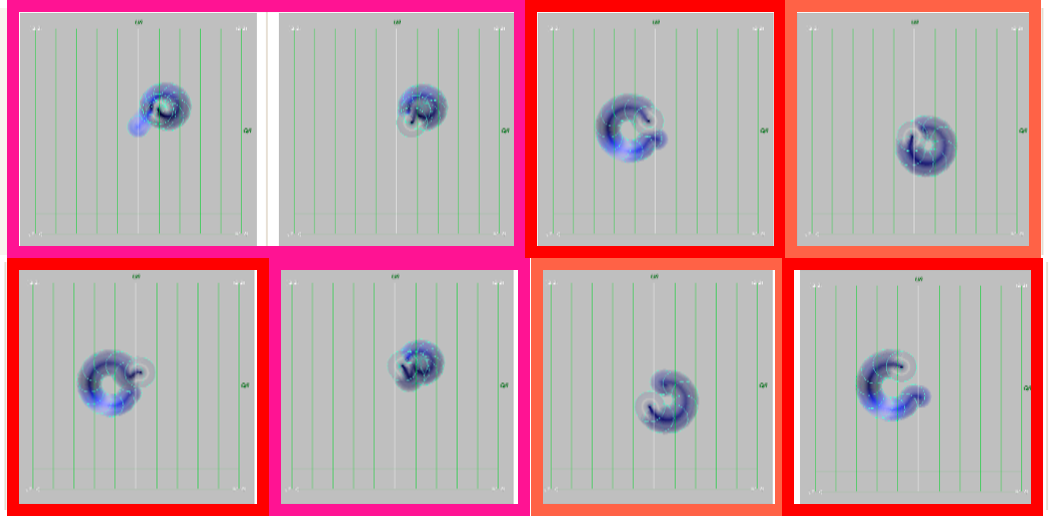
\includegraphics[width=.99\linewidth]{figures/QBSResultsResultQuery_revised.png}\\
        \footnotesize{\sf (d)~Results for the query in (b).}
    \end{minipage}
    \caption{QBS results for our synthetic dataset in Fig.~\ref{fig:synthesisData}.
        On the basis of a hand-drawn sketch in (a), an unexpected result is highly ranked (white outline) in (c). 
        With a sketch based on actual data values (b), no unexpected results appear, as illustrated in (d).
        }
    \label{fig:QBSDemodata}
\end{figure}
\textsf{Experimental results.\ } We evaluated the effectiveness of our QBS method using our synthetic data.
First, we sketched a pattern shown in Fig.~\ref{fig:QBSDemodata}~(a) to extract time intervals with small circular patterns.
The sketch pad plane corresponds to the Stokes plane, and for simplicity, the stroke width is not used.
To detect time intervals with a similar shape but different positions or scales, we used the normalization and polar coordinates options.
Fig.~\ref{fig:QBSDemodata}~(c) shows the top eight results for our QBS in (a).
The outline color of each thumbnails matches the color of the corresponding pattern in Fig.~\ref{fig:synthesisData}~(b).
All three time intervals highlighted in red in Fig.~\ref{fig:synthesisData}~(b) were precisely extracted.
However, an unexpected result (i.e., the thumbnail with white outline in Fig.~\ref{fig:synthesisData}~(c)) was highly ranked as a candidate similar to the input sketch due to the ambiguities of the hand-drawn sketch.
We address this problem by incorporating fact-guided querying (see Section~\ref{sec:factDrivenQuerying}). 

\subsection{Query Matching Algorithm}\label{sec:matchingAlgorithm}
There are many different methods for computing the distance between two time series, such as Euclidean distance, uniform scaling, and dynamic time warping (DTW)~\cite{Berndt1994}.
TimeTubesX uses DTW
because it aligns two time series elastically and thus supports the comparison of time series with different lengths.
Additionally, it can compute the distance between two time series that are similar but locally out of phase.
%more intuitively even if they are out of phase in the time direction. 
According to Eichmann and Zgraggen~\cite{Eichmann2015}, the DTW similarity measurement seems to most closely match human perception.
There are multiple solutions for dealing with multi-dimensional data in DTW. 
TimeTubesX implements two options, ${\rm DTW}_{\rm I}$ (independent) and ${\rm DTW}_{\rm D}$ (dependent), both of which are based on the work of Shokoohi-Yekta et al.~\cite{Shokoohi-Yekta2015}.

${\rm DTW}_{\rm I}$ computes the distance between two time series for each dimension of the data separately. 
In the final step, it adds up all the individual distances to produce the final distance measure.
Consequently, this approach focuses more on the similarity of each dimension and less on correlations between different dimensions.
${\rm DTW}_{\rm D}$, on the other hand, computes the distance between two data samples directly over all dimensions (i.e., as Euclidean distance in $n$-dimensional space).
Therefore, this method focuses more on correlations among the different dimensions of a time series and less on the similarities of individual dimensions. 
By default, our system uses ${\rm DTW}_{\rm D}$ because correlations among variables are important for blazar behavior analysis.
Readers are recommended to consult \cite[Fig. 1]{Shokoohi-Yekta2015} for comprehensive illustrations of ${\rm DTW}_{\rm I}$ and ${\rm DTW}_{\rm D}$.
We use a sliding window approach in our matching algorithm.
Users can set the window size and the step size of the sliding window and also set a constraint on the largest allowed temporal shift (i.e., warping window size)
in the process of finding the best alignment between the query and time series.
Users can specify these parameters at the bottom of the query specification panel in Fig.~\ref{fig:UIFeatureExtraction}~(A).
Note that multiple time intervals with different lengths but that include the same data samples can be presented in the extraction results (see Fig.~\ref{fig:QBEDemodata} and Fig.~\ref{fig:QBSDemodata}~(c) and (d)).
The timelines in Fig.~\ref{fig:UIFeatureExtraction}~(C) help users recognize such time intervals. 

Normalization and polar coordinates options enable a fuzzy pattern search.
The normalization option instructs the system to normalize a query and time intervals into the range of $[0, 1]$.
Subsequently, the pattern search places great significance on the shape of the time variations, whereas the actual value ranges will be ignored.
With the polar coordinates option, 
$q(t)$ and $u(t)$ are converted into polar coordinates ($r-\theta$ domain) before computing similarities.
Subsequently, the pattern search with the normalization and polar coordinates options will also be able to extract patterns rotating around the origin of the Stoke plane.

\subsection{Fact-Guided Querying}\label{sec:factDrivenQuerying}
To support quick and iterative query refinement, TimeTubesX allows users to re-utilize individual extraction results as an input for follow-up queries, a process we have termed \emph{fact-guided querying}.
By iteratively updating a query, users can, in a step-by-step manner, identify more observable time intervals that reflect their intentions.
Therefore, fact-guided querying contributes immensely to drilling down into data as a part of the visual exploration framework of TimeTubesX in Fig.~\ref{fig:framework}.
In QBE, users can switch variables used in the matching process and modify the time range of the query, while in QBS, users can adjust the scale, shape, and axis of the input query or add further filtering constraints.
Thus, fact-guided querying helps users perform further pattern searches based on a time interval of interest found in the previous process or create a sketch-based query from references to actual data measurements instead of from a blank sketch pad.

Our system allows users to build a fact-guided query with simple interactions by, for example, dragging an extraction result either into the QBE interface (part (2) in Fig.~\ref{fig:querySpecificationPanel}~(B)) or into the sketch pad of the QBS interface (part (3) in Fig.~\ref{fig:querySpecificationPanel}~(C)).

\textsf{Experimental results.\ } We confirmed the usefulness of the fact-guided querying approach with our synthetic data.
As discussed in Section~\ref{sec:QBS}, 
hand-drawn sketch queries, such as Fig.~\ref{fig:QBSDemodata}~(a), work well for finding time intervals with a specific feature,
but ambiguities of hand-drawn sketches may sometimes lead to unexpected results, as shown in (c).
If the extraction results for the query in (a) sufficiently represent users' intentions, one of the results can be used as an input to refine the results of the next visual query.
We chose the top left result of Fig.~\ref{fig:QBSDemodata}~(c) and used it as an input for our QBS method, as shown in (b). 
The sketch pad plane in (b) coincides with the Stokes plane.
Thereafter, we ran QBS using the same parameter settings as the example in Section~\ref{sec:QBS}.
As shown in the top eight extraction results in (d),  
this refined query in (b) no longer produces any high-ranking outliers or unexpected results.